\documentclass{IEEEtran}

\usepackage[utf8]{inputenc}
\usepackage{graphicx}
\usepackage[spanish]{babel}
\usepackage{authblk}
\usepackage[T1]{fontenc}

\begin{document}

	\title{Sistema de monitoreo de lactantes durante el sueño para la disminución del síndrome de muerte súbita}
	\author{Diego Bertolini, Filippo Comandini, Universidad de Palermo}
	\date{Mayo de 2018}	
	\maketitle
	
	\begin{abstract}
		Desarrollo de un dispositivo que realice la tarea de monitorear a un bebé durante las horas de sueño a través de distintos sensores los cuales permitirían controlar la respiración, movimiento y temperatura entre otros, incorporados a una cuna o sector donde descansa el lactante, y con un costo de fabricación muy bajo. Además incorpora una forma de alerta hacia los padres o tutores ante la detección de variaciones drásticas en los distintos indicadores de datos que se toman desde los sensores y serán visualizados a través de una aplicación móvil.
	\end{abstract}
	
	Palabras clave: alertas, bebé, lactante, muerte súbita.
	
	Nomenclaturas: aplicación móvil, Arduino.
	
	\section{Introducción}
	
		\fontfamily{pcr}
	
		El síndrome de muerte súbita en el lactante \textbf{(SMSL)} \cite{garcia2008sindrome} se define como la muerte repentina, inesperada y sorpresiva de un niño generalmente menor de un año de edad, que si bien la muerte súbita no es exclusiva del lactante ya que puede presentarse en niños mayores, jóvenes y adultos, pero en la mayoría de los casos se da en el lactante y es hacia ese enfoque en donde se desarrolla el presente trabajo de investigación. Los padres primerizos enfrentan con mucho temor los primeros meses de vida de un hijo, pues es en esa época en donde se presentan situaciones desesperantes en el cuidado del recién nacido con el conocido síndrome de muerte súbita. Pueden encontrarse ciertos factores de referencia del síndrome y recomendaciones \cite{subita2000nuevas} para evitarlo. El estudio de su ambiente en donde ocurren estos casos es fundamental para encontrar distintos tipos de riesgos que pudieran reducirse \cite{aguilera2002importancia}.
		
		Se han desarrollado una serie de dispositivos que permitirían la reducción significativa del número de muertes producidas por dicha problemática. Existen investigaciones previas, por ejemplo en los trabajos \cite{teodorescu2000respiration} y \cite{hafner2007non} donde requiere la utilización de un Baby Monitor tradicional y un dispositivo radar Doopler para el monitoreo de la actividad cardiopulmonar, u otros casos \cite{brady2005garment} o \cite{lee2012baby} en donde se basan en el monitoreo del ritmo de respiración basado en prendas de vestir en un diagnóstico de 10 minutos. Estos proyectos implican un costo mayor al que es implementado en la presentación actual, o incluso con monitores que implican tener cierto tipo de contacto invasivo con el lactante y colocación del mismo previo a la toma de mediciones. 
		
		El presente proyecto representa una forma muy económica de monitorear al bebé y de una forma que no requiera invasión por contacto o atención de colocación de dispositivos previo al sueño, acompañando de esta forma al simple estilo de vida normal llevado adelante por los padres y tutores.

	\section{Casos de estudio}

		En ésta sección se mencionan los aspectos principales a ser estudiados dentro del entorno en el cual se desarrolla la actividad diaria en cada hogar con respecto al área donde descansa el bebé, para así obtener datos específicos y reducir riesgos. Las áreas de estudio se describen como por ejemplo la cuna donde descansa el bebé, el posicionamiento del lactante dentro del área de estudio, la temperatura corporal, la respiración y sus movimientos.

		El cuidado de bebés durante las horas de sueño es un proceso altamente demandante y estresante en tiempo para las personas a cargo. La tarea incluye el control de ciertos factores que determinan el bien estar del bebé y el análisis de disminución de riesgos ante tragedias de muerte súbita durante ese proceso. En el ambiente en el que se encuentra existen variables como la luz, temperatura, humedad, ruido e incluso la calidad del aire o la ausencia de determinados gases que pueden ser dañinos para un bebé. El objetivo del presente proyecto es analizar datos obtenidos por los sensores dentro del ambiente en el cuál se van a enfocar en el movimiento, respiración y temperatura del bebé, para así identificar emergencias que pueden ser causadas por episodios que desencadenen en una muerte súbita por obstrucción de las vías respiratorias, ante los cambios drásticos de los indicadores o variables ambientales.
		
		El proyecto se focaliza en realizar el control de estas variables, facilitando la tarea de las personas a cargo en cuando al control que realizan noche tras noche y ofreciendo mayor tranquilidad en el cuidado. Esta tecnología nos permite identificar episodios en los cuales comprometen la salud del bebé ya sea por movimientos que puedan generar una obstrucción en las vías respiratorias, vómitos durante la noche y en una posición comprometida, posibles casos epilépticos con un exceso de movimiento, para finalmente notificar a las personas encargadas del cuidado del lactante y tomar medidas inmediatas.

		\subsection{Cuna o área analizada}

			Desde su nacimiento hasta algunos meses después, los bebés tienen los músculos poco desarrollados como para poder evitar posiciones o incidentes indeseados que generen desenlaces dramáticos. La cuna es el principal lugar donde el bebé descansa y pasa la mayor parte del día, y en donde los padres o tutores pierden la atención mayor cantidad del tiempo sobre todo por las noches. A través del tiempo se hicieron cambios en el diseño de las cunas para mejorar la calidad de vida de los pequeños, ya sea haciéndolas más ergonómicas, previniendo malas posturas y hasta utilizando ingeniería en materiales para evitar el desarrollo de agentes biológicos que pueden ser dañinos para seres humanos sin un sistema inmunológico completamente desarrollado. La utilización de materiales indicados en la construcción de una cuna son altamente demandados, al igual que pinturas y adornos no tóxicos, ya que es inevitable que un bebe ocasionalmente se lleve a la boca y muerda lo que tiene a su alcance. Siguiendo estos lineamientos de cuidado para los recién nacidos, este proyecto realiza la implementación de un sistema de sensores a estas cunas, sin entrar en contacto directo con el bebé como por ejemplo en la cita \cite{broussard2002baby}.
		
		\subsection{Posicionamiento dentro del área de estudio}

			La idea principal de éste análisis es el de determinar si el cuerpo del bebé se encuentra dentro de la zona de estudio, de manera tal de determinar si el sistema está en condiciones de realizar los monitoreos pertinentes o bien notificar hacia las personas responsables sobre el incidente detectado, que pudiera ser causado o no por el movimiento del lactante en un desplazamiento sobre la cuna. La funcionalidad sobre la detección del bebé dentro de la zona de estudio se basa en la habilitación de los sensores correspondientes para la toma de información, es decir que si el sistema detecta la ausencia del lactante, los indicadores recolectados tanto de temperatura o movimiento estarían fallando en los datos obtenidos, por lo tanto dichos indicadores deberían ser descartados.
		
		\subsection{Temperatura corporal}

			La temperatura del bebé debe ser controlada, no solo por cuestiones de determinar o ayudar a la toma de estadísticas que hagan al disparo de alertas por problemas, como también para llevar un control periódico. De ésta forma los tutores, padres o responsables pudieran llegar a analizar a lo largo del tiempo, por datos almacenados en un período de tiempo, la fluctuación de los valores, detectar si existe una elevación de su temperatura para detectar fiebres, o incluso la perdida del calor corporal por otras causas.

		\subsection{Respiración}

			La respiración es uno de los factores o indicadores principales en los cuales se va a enfocar este sistema. Uno de los principales problemas que causan el SMSL son causados por los movimientos nocturnos que dejan mal posicionados al bebé generando una obstrucción en las vías respiratorias. De misma manera ocurre en otras incidencias causadas por vómitos nocturnos con el bebé posicionado en una forma desfavorable para le expulsión completa de los líquidos segregados, causando así también una obstrucción en las vías respiratorias.

			La idea es que mediante ciertos sensores incorporados en el lugar de la conciliación del sueño se pueda detectar la constante vibración causada por los movimientos de respiración del lactante. La necesidad de contar con sensores altamente sensibles es indispensable para la detección satisfactoria de la vibración causada por la respiración sobre la superficie donde duerme el lactante. A lo largo de la investigación de éste trabajo se han encontrado diferentes proyectos que contemplan el análisis de estos parámetros de entrada, desde plataformas posicionadas por debajo del bebé, hasta dispositivos colocados en prendas de vestir o cinturones colocados en el abdomen. Una de las formas que se van a implementar para el presente trabajo de investigación reside en una plataforma que está posicionada debajo del lactante, de forma tal de tomar los indicadores o mediciones requeridas de la manera menos invasiva y natural posible.

			También es importante destacar que ante la lectura del posicionamiento del bebé dentro del área de estudio, éste indicador podría estar arrojando un valor nulo, o dicho con otras palabras, indicando como si no estuviera detectando respiración del bebé, es por ello que es importante la detección del cuerpo dentro del área de estudio y en tal caso descartar la información obtenida.
	
		\subsection{Movimientos}

			Uno de los objetivos principales del proyecto es el de monitorear el movimiento del bebé cuando está recostado sobre su cuna o el lugar indicado para conciliar el sueño. El objetivo reside en analizar si el movimiento es alto a tal punto de considerar si es conveniente realizar un análisis exhaustivo del sueño referido al movimiento, siendo éste un indicador a modo informativo para comportamientos. El movimiento puede detectarse de forma activa o pasiva. Cuando un sensor emite algún tipo de energía se trata de una detección activa, mientras que cuando el sensor no emite ningún tipo de energía, se trata de una detección pasiva.

	\section{Hardware}

		La presente sección tiene como objetivo principal mencionar cuáles son los ítem principales y fundamentales que entran en funcionamiento para la resolución de la problemática. Los distintos módulos corresponden a una serie de herramientas y posteriores desarrollos que harán al funcionamiento del sistema en su totalidad y visualización hacia el usuario final. Los ítem tratados van desde la plaqueta Arduino, sensores, conectividades, hasta incluso el software de aplicación móvil.

		\subsection{Esquema general}

			El marco general del sistema a implementar está comprendido por un hardware constituido por una plaqueta Arduino y sus sensores correspondientes para tomar los indicadores necesarios conectados a la plaqueta Arduino principal para procesar toda la información, y una aplicación móvil, instalada en un dispositivo como un teléfono celular o tablet, en donde se visualiza la información recolectada y arrojar alertas si corresponde. La conectividad entre la plaqueta Arduino y la aplicación móvil se realiza mediante un módulo Bluetooth, la comunicación se realiza punto a punto con envío y recepción de un buffer de datos que será interpretado según corresponda. En la \textbf{Figura \ref{esquemageneral}} se puede observar un diagrama del esquema anteriormente mencionado y todos sus módulos incorporados.

			\begin{figure}
				\centering
				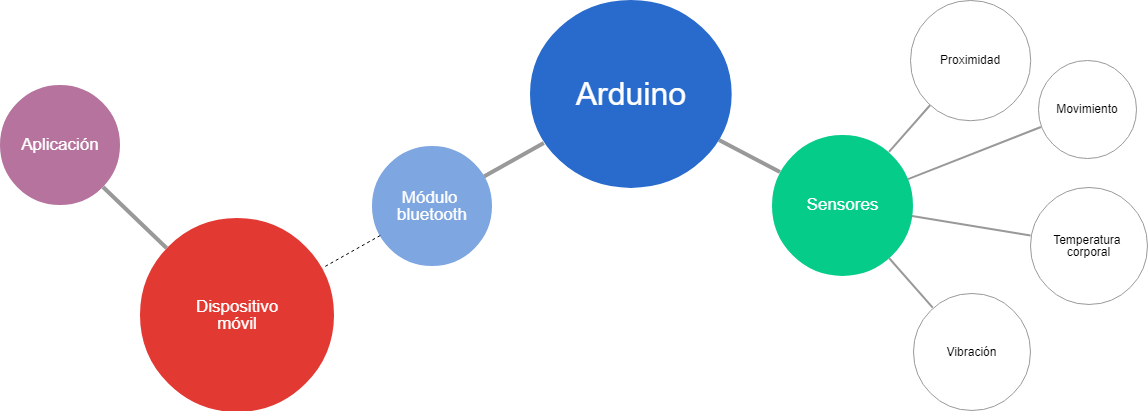
\includegraphics[width=1\linewidth]{esquemageneral}
				\caption{Esquema general}
				\label{esquemageneral}
			\end{figure}

		\subsection{Arduino}

			Gracias al avance tecnológico, hoy en día podemos contar con dispositivos pre-diseñados que nos ayudan en los desarrollos ahorrando mucho tiempo y costos. Es el caso de Arduino \cite{arduinourl} que desarrolló una plaqueta que cumple la función de un micro-controlador programable.
			Como se puede apreciar en la \textbf{Figura \ref{arduino-mega}}, se estará utilizando la versión Mega 2560 de Arduino, en donde los distintos módulos requeridos serán conectados a través de sus pines de entrada y salida (analógico y/o digital) que se pueden observar. El lenguaje de programación utilizado es C++ \cite{arduinocode}. 

			\begin{figure}
				\centering
				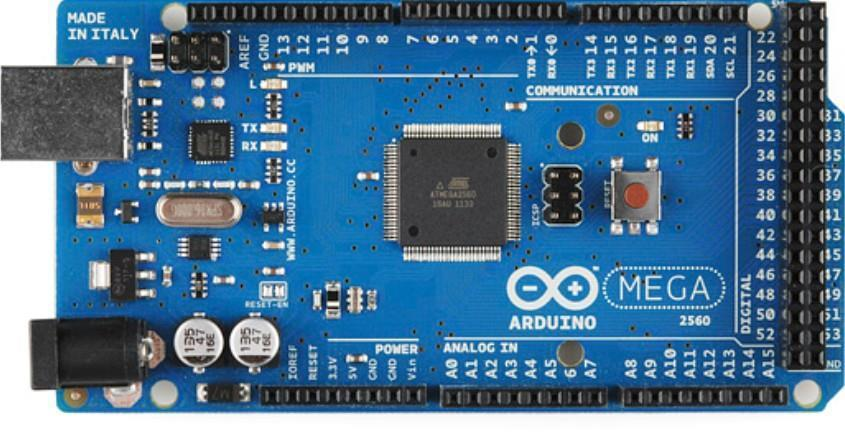
\includegraphics[width=0.8\linewidth]{arduino-mega}
				\caption{Arduino MEGA 2560}
				\label{arduino-mega}
			\end{figure}

		\subsection{Sensores}

			\subsubsection{Módulo sensor de proximidad (\textbf{IR FC-51})}

				El sensor representado en la \textbf{Figura \ref{arduino-modulo-proximidad}} detecta interposición de algún objeto entre una distancia pre-configurada y el mismo (sin contacto, entre una distancia de 2 cm a 30 cm, y con un ángulo de detección de 35º) \cite{proximidadtecnico}. La utilidad de éste sensor se verá reflejada ante la necesidad de detectar si el bebé se encuentra dentro del área de estudio de donde se obtendrían los datos de los otros sensores incorporados, o si el sistema debiera descartar los datos obtenidos o mismo desactivar los sensores ante la ausencia del bebé en el área e informar hacia la aplicación móvil. El sensor funciona mediante la transmisión de ondas o impulsos infrarrojos los cuales son transmitidos hacia la dirección aproximada donde se dirige el mismo, y recibe las ondas que rebotan en determinados objetos en caso de haberlos, es decir que trabaja sobre la reflexión de luz infrarroja. El presente módulo cuenta con un potenciómetro el cual regula la sensibilidad de las detecciones, pudiéndose traducirse como sensibilidad de distancia de objetos. 

				\begin{figure}
					\centering
					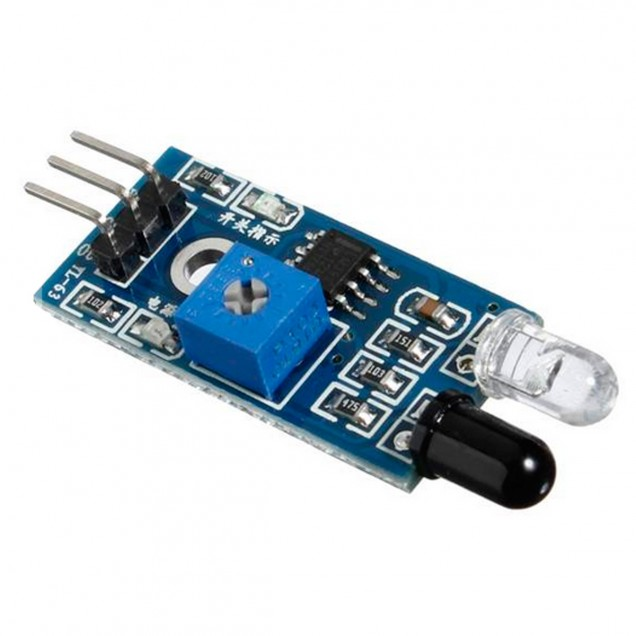
\includegraphics[width=0.5\linewidth]{arduino-modulo-proximidad}
					\caption{Módulo de proximidad infrarrojo IR FC-51 para Arduino}
					\label{arduino-modulo-proximidad}
				\end{figure}

			\subsubsection{Módulo sensor de temperatura direccional (\textbf{MLX90614})}
			
				Es un sensor de temperatura direccional sin contacto y con incidencia hacia un cierto rango de distancia entre el objeto observado y el sensor mismo \cite{temperaturatecnico}. Una imagen del sensor mencionado se puede observar en la \textbf{Figura \ref{arduino-modulo-temperatura}} y será el encargado de obtener la temperatura corporal del lactante al direccionarse hacia donde se presupone va a estar posicionada la cabeza del bebé, de forma tal que el indicador obtenido por dicho sensor sea lo más certero posible.

				\begin{figure}
					\centering
					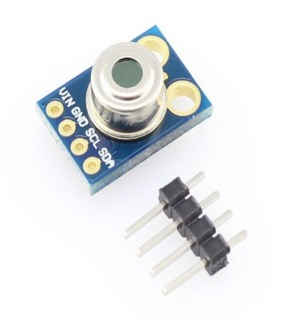
\includegraphics[width=0.5\linewidth]{arduino-modulo-temperatura}
					\caption{Módulo de temperatura direccional MLX90614 para Arduino}
					\label{arduino-modulo-temperatura}
				\end{figure}

			\subsubsection{Módulo sensor de vibración (\textbf{AA2758})}
			
				Sensor analógico que se basa en un mecanismo de cerámica entre placas metálicas, comúnmente denominado piezoeléctrico, el cual reacciona ante vibraciones generando señales eléctricas que son obtenidas y enviadas a la placa Arduino para su posterior manipulación o interpretación. El objetivo de éste sensor es el de obtener movimientos y vibraciones que sean localizados por debajo del bebé a través de una red de piezoeléctricos. Con la sensibilidad adecuada y la interpretación de los datos obtenidos se puede realizar un control sobre la respiración del bebé ante la variación de presión por el movimiento toráxico que esto implica. En la \textbf{Figura \ref{arduino-modulo-vibracion}} se observa el módulo correspondiente y el piezoeléctrico conectado al mismo.

				\begin{figure}
					\centering
					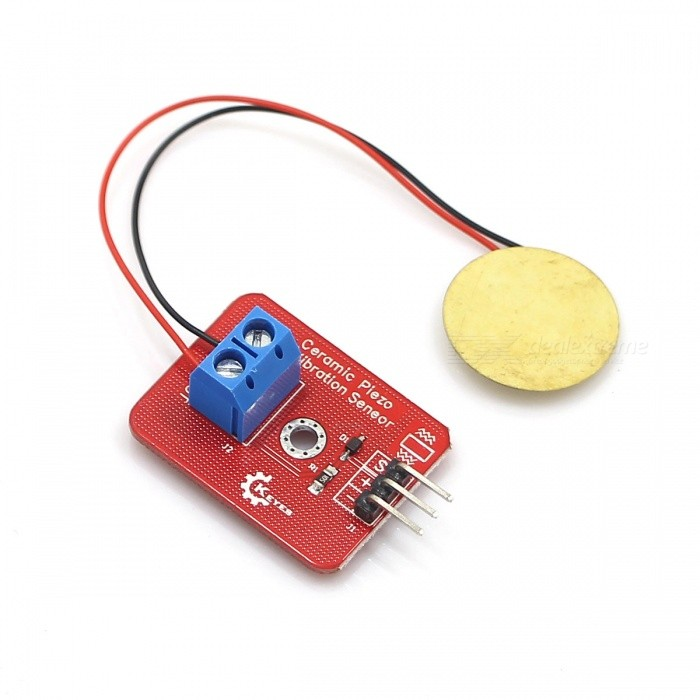
\includegraphics[width=0.5\linewidth]{arduino-modulo-vibracion}
					\caption{Módulo sensor de vibración AA2758 para Arduino}
					\label{arduino-modulo-vibracion}
				\end{figure}

			\subsubsection{Módulo sensor de movimiento (\textbf{HC-SR501})}
			
				Módulo el cual integra un sensor PIR (Passive Infrared), generalmente utilizado para sistemas de alarma en la detección de movimiento \cite{movimientotecnico}. La principal función de éste módulo radica en medir la cantidad de movimiento durante el sueño del lactante y detectar cuales son los horarios en que podría despertarse durante la noche. Además indicaría cuáles son aquellos ciclos en donde el bebé pudo haberse movido de alguna manera ocasionando una modificación en la postura en la que fue colocado y pudiendo obstruir las vías respiratorias. En la \textbf{Figura \ref{arduino-modulo-movimiento}} se puede observar el módulo sensor de detección de movimiento.

				\begin{figure}
					\centering
					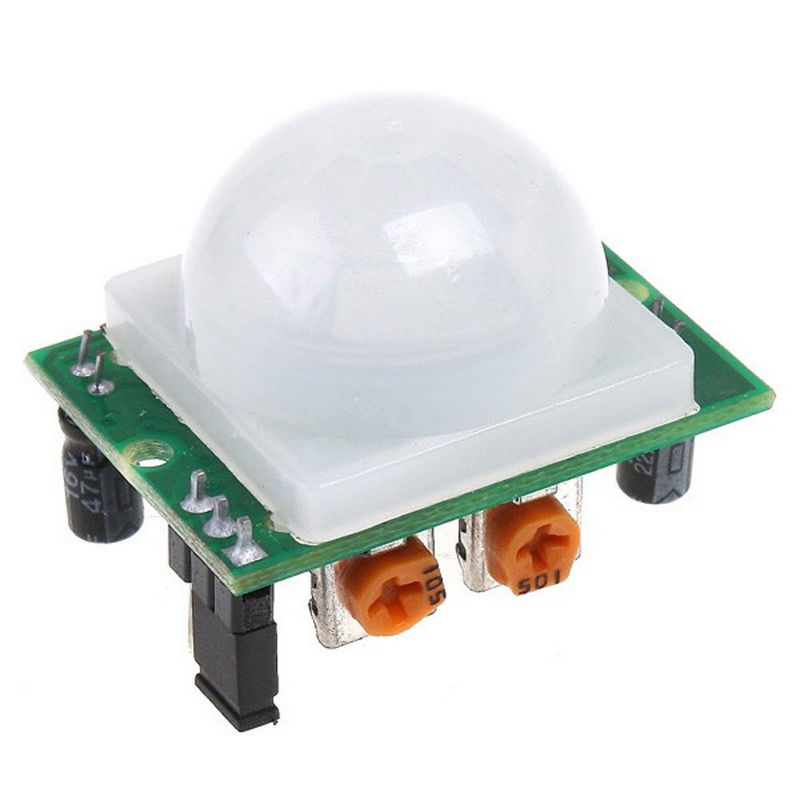
\includegraphics[width=0.5\linewidth]{arduino-modulo-movimiento}
					\caption{Módulo sensor de movimiento HC-SR501 para Arduino}
					\label{arduino-modulo-movimiento}
				\end{figure}

		\subsection{Módulo de comunicación (\textbf{HC-06})}

			Es otro de los módulos más importantes que tiene el sistema ya que es el encargado de comunicarse inalámbricamente con el dispositivo móvil, cuya aplicación está instalada, y así transmitir datos, visualizar indicadores y alertar ante cualquier incidente que pudiese ocurrir que ponga en riesgo la vida del bebé. El módulo mencionado realiza una conexión punto a punto entre la plaqueta Arduino que recolecta toda la información y el dispositivo móvil (teléfono celular o tablet) que tiene la aplicación. Es importante destacar que éste módulo trabaja con una tecnología de Bluetooth tradicional y no BLE, con lo que representa una incompatibilidad con los dispositivos de Apple. En la \textbf{Figura \ref{arduino-modulo-bluetooth}} se puede observar el módulo de comunicación Bluetooth mencionado.

			\begin{figure}
				\centering
				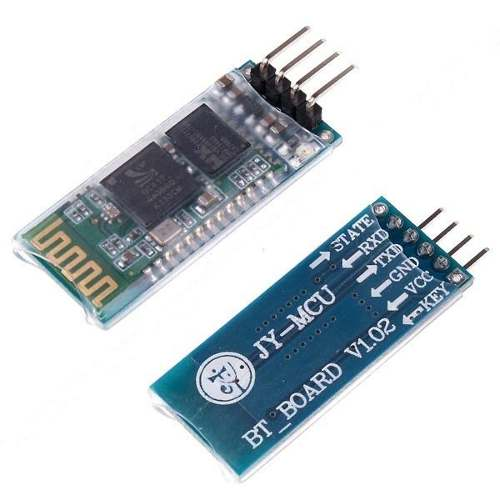
\includegraphics[width=0.5\linewidth]{arduino-modulo-bluetooth}
				\caption{Módulo de comunicación Bluetooth HC-06}
				\label{arduino-modulo-bluetooth}
			\end{figure}

		\subsection{Aplicación móvil}
		
			El uso de los dispositivos móviles es algo que ya forma parte de nuestra cultura diaria, y es por ello que el proyecto presentado tiene relación a la conectividad móvil, ya que es posible hacer llegar la información leída por los sensores a dispositivos móviles, permitiendo estar en contacto permanente con el estado de las diferentes variables ambientales que rodean y afectan al bebé, pudiendo inferir en el bienestar del mismo. Las alertas o notificaciones emitidas por la aplicación son producto de parámetros que varían a través del tiempo, identificando los cambios abruptos de los mismos indicando algún cambio de estado. 
			
			En este proyecto la aplicación móvil estará desarrollada tanto para la plataforma Android como iOS, pero cabe destacar que la compatibilidad del hardware de las plataformas mencionadas y el módulo de conectividad Bluetooth utilizada solamente es viable con dispositivos Android, ya que los dispositivos iOS utilizan otro tipo de tecnología conocida como BLE (Bluetooth Low Energy).
			El desarrollo del aplicativo estará basado sobre Ionic, el cual es un framework diseñado para el desarrollo de aplicaciones móviles híbridas, el cual se basa en Angular, Typescript, Javascript, CSS3 y HTML5. El concepto principal se basa en la traducción gráfica de todos los componentes visualizados en cada dispositivo móvil dependiendo la plataforma en la cual se encuentre, ya sea para Android o para iOS, cada componente utilizado tiene su representación gráfica acorde a la plataforma.
			Uno de los principales pilares que tiene Ionic es el de incorporar las librerías de Apache Cordova, la cual contiene toda la lógica, o motor principal, para traducir el código desarrollado independiente por cada plataforma. Es decir, Cordova contiene los desarrollos individuales, algunos desarrollados oficialmente y otros por grupos de desarrolladores de la comunidad que hacen su aporte, de los plugins que hacen a la funcionalidad de cada módulo del sistema operativo en cuestión. En la \textbf{Figura \ref{ionic-angular-cordova}} se puede observar cómo interactúan los distintos componentes que hacen al desarrollo de la plataforma final distribuida para cada sistema operativo.

			\begin{figure}
				\centering
				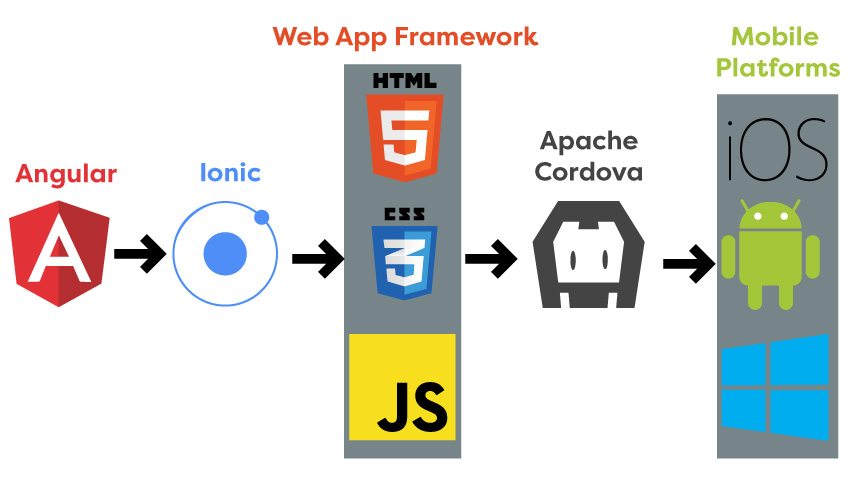
\includegraphics[width=1\linewidth]{ionic-angular-cordova}
				\caption{Esquema de arquitecturas Ionic - Angular - Cordova}
				\label{ionic-angular-cordova}
			\end{figure}

			En lo que respecta al desarrollo híbrido, el aplicativo final para cada plataforma, se traduce como un navegador web incorporado el cual es visualizado por el usuario final. Es por ello que el desarrollo principal está hecho sobre plataformas web. En la \textbf{Figura \ref{ionic-angular-cordova-webview}} se observa el componente WebView que interpreta los recursos incorporados y los lenguajes HTML, CSS y Javascript, dicho componente es el que simula un navegador web dentro del aplicativo final.

			\begin{figure}
				\centering
				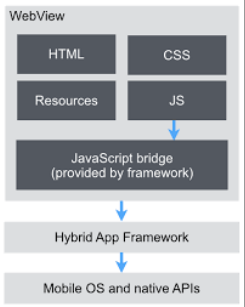
\includegraphics[width=0.6\linewidth]{ionic-angular-cordova-webview}
				\caption{Componentes internos Cordova}
				\label{ionic-angular-cordova-webview}
			\end{figure}
			
	\section{Desarrollo}

		En ésta sección se estará comentando cuáles fueron los lineamientos principales para el desarrollo contemplando códigos y frameworks utilizados para hacer a la solución en su plenitud. Se mostrarán imágenes de las mediciones obtenidas por cada sensor a través del software Telemetry Viewer mencionado, la aplicación final con los indicadores y alertas deseadas, y cómo fue el desarrollo o traspaso de información entre la plataforma hardware y el software para llegar hacia el usuario final.

		El dispositivo que realizará la función de monitoreo al lactante se concentra en un hardware que no es invasivo para el mismo. Los sistemas de medición que se aplican, es decir, los diferentes sensores que toman datos del lactante, no deben tener contacto directo con el mismo. De esta forma la forma y estructura de funcionamiento será lo más normal y natural cotidiano que se encuentra día tras día en los hogares. En la investigación previa a la realización del presente documento se han encontrado diferentes sistemas ya creados a nivel mundial, los cuales algunos de ellos requieren algún tipo de contacto exclusivo con la piel del bebé, como por ejemplo en aquellos dispositivos que son incorporados en la vestimenta, obligando a los padres y/o tutores a tomar ciertas medidas previas a la colocación del bebé en la cuna las cuales se pueden llegar a tornar medias tediosas o directamente ser rechazadas por los responsables al ser un tanto invasivas. También en la investigación se han encontrado algunos dispositivos los cuales no tienen contacto directo con el lactante, los cuales fueron tomados de ejemplo y estudio para generar el dispositivo actual con distintos valores agregados.

		\subsection{Metodología y mediciones}
			
			Para capturar los valores recibidos por los distintos sensores incorporados se utilizó una herramienta gráfica en vivo llamada Telemetry Viewer \cite{telemetryviewer} la cual se basa en los valores arrojados por la placa Arduino a través del serial. Cada valor enviado por el Arduino es separado por comas, y luego cada uno de ellos conociendo el orden visualizado será tomado por Telemetry Viewer adaptado a la visualización deseada. A continuación se realiza una demostración de los valores arrojados por los sensores que toman los datos del ambiente, exceptuando el módulo de comunicación Bluetooth:

			\subsubsection{Módulo sensor de proximidad}

				En la \textbf{Figura \ref{proximidad}} se observa el gráfico arrojado por los valores obtenidos por el sensor. A través de una linea de tiempo se visualiza un salto inmediato hacia un valor constante de acuerdo a la detección del sensor, es decir que aquellos saltos son marcados cuando el sensor detecta un objeto dentro del área de inspección, caso contrario vuelve a su estado de reposo inmediatamente.
				\begin{figure}
					\centering
					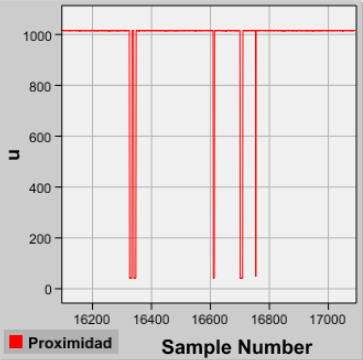
\includegraphics[width=0.6\linewidth]{proximidad}
					\caption{Datos del sensor de proximidad}
					\label{proximidad}
				\end{figure}

			\subsubsection{Módulo sensor de temperatura direccional}

				En la \textbf{Figura \ref{temperatura}} se expresa en un gráfico del tipo acelerómetro el indicador correspondiente a la temperatura. El indicador aumenta o disminuye dinámicamente lo que corresponde a la lectura de la temperatura corporal del bebé adquirida. El valor arrojado está expresado en grados centígrados.

				\begin{figure}
					\centering
					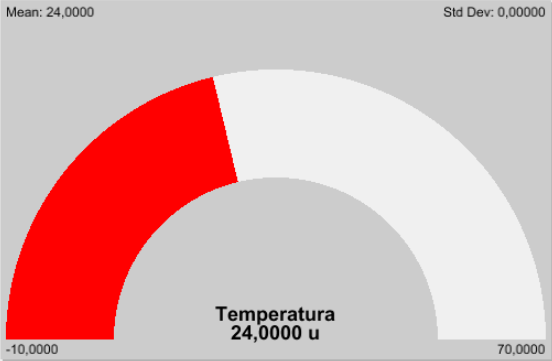
\includegraphics[width=0.7\linewidth]{temperatura}
					\caption{Datos del sensor de temperatura}
					\label{temperatura}
				\end{figure}

			\subsubsection{Módulo sensor de vibración}

				En la \textbf{Figura \ref{piezo}} se puede observar el gráfico del sensor de vibración en la cual se ve como reacciona la variación de valores desde su estado de reposo según movimientos o vibraciones detectadas. Los datos arrojados y visualizados en el gráfico representa un indicador de voltaje en la placa cerámica del piezoeléctrico el cual varía a través del tiempo según vibraciones detectadas. 

				\begin{figure}
					\centering
					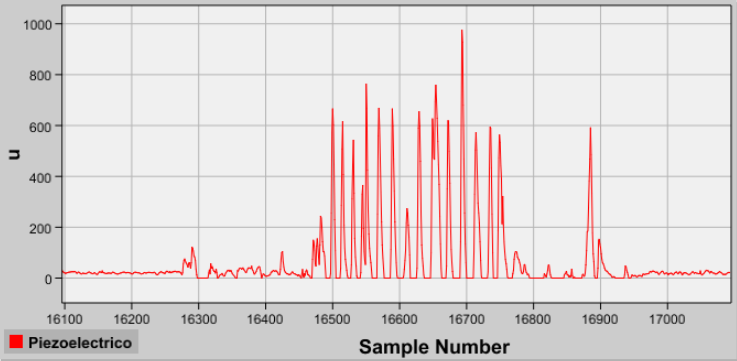
\includegraphics[width=1\linewidth]{piezo}
					\caption{Datos del sensor de vibración}
					\label{piezo}
				\end{figure}

			\subsubsection{Módulo sensor de movimiento}
				
				Similar al sensor de proximidad anteriormente mencionado, al detectar una variación de radiación en los distintos campos o espectros del sensor, se produce un salto desde su estado de reposo hacia un valor constante de forma inmediata. La diferencia que reside en este sensor es que a través de la linea de tiempo en la cual transcurren los saltos de valores, los mismos se mantienen en un corto lapso de tiempo para volver a recalibrar el estado de reposo del mismo. Se puede observar en la \textbf{Figura \ref{movimiento}} el indicador mencionado y sus valores.

				\begin{figure}
					\centering
					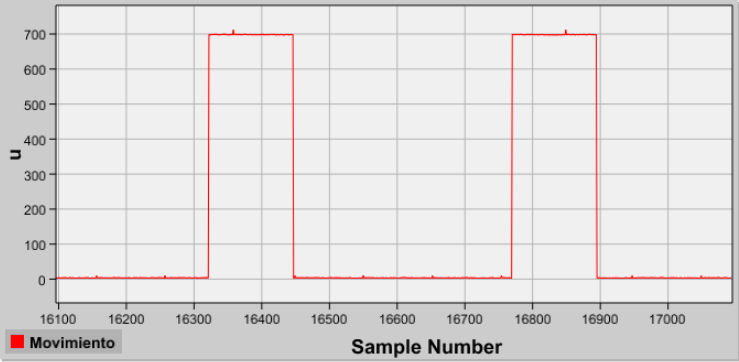
\includegraphics[width=1\linewidth]{movimiento}
					\caption{Datos del detector de movimiento}
					\label{movimiento}
				\end{figure}

		\subsection{Visualización y alertas}

			La parametrización de los valores resulta importante para la detección de las alertas a ser enviadas al usuario. La aplicación permite la configuración a gusto según el criterio de cada usuario permitiendo distintos niveles de sensibilidad a la hora de aplicar el algoritmo que dispare la alarma en cuestión. En caso de que los valores indicadores captados por los sensores estén por fuera de esos valores mínimos y máximos, inmediatamente se disparará una alerta sonora y visual según del sensor que se tratase.

	\section{Conclusión}

		El dispositivo final aprovecha la tecnología comercialmente accesible de hoy en dia para tomar datos sensoriales del bebé y obtener datos que resultan útiles para las personas a cargo del cuidado de los pequeños. Si bien el avance de la tecnología hará que se lancen nuevos sensores al mercado, la modularización del sistema nos da gran libertad para reemplazarlos y probar nuevas versiones. La elección de Arduino Mega para el prototipo nos da esta flexibilidad, aunque la posibilidad de utilizar otro tipo de placa madre, como por ejemplo una Raspberry pi, para incorporar esos nuevos sensores queda abierta al cambio.
		Una vez lograda la comunicación entre Arduino y la aplicación móvil, se pudieron procesar los datos para identificar posibles situaciones de riesgo y emitir alertas acordes a ellas, de forma tal que dar una alerta temprana sobre una situación crítica podría salvar la vida del bebé. El análisis realizado sobre los datos es directo, aunque es posible la integración futura sobre el campo de inteligencia artificial para tomar decisiones en base al aprendizaje de los datos obtenidos por los sensores, ya sea aplicado para emitir notificaciones futuras en base a predicciones u otras aplicaciones.

		\subsection{Mejoras}

			Una de las mejores adaptaciones que pueden integrarse al presente dispositivo corresponde a la adaptación hacia una incubadora, de forma tal que mediante una serie de dispositivos aplicados en sectores de la salud pública y privada, se podría monitorizar a un grupo de bebés que estén en los hospitales o clínicas y ayuden al control de ellos. A su vez lo que respecta a la conectividad inalámbrica, se podría migrar hacia una conectividad mediante módulos Wifi para lograr el monitoreo remoto sin necesidad de estar cerca y con información disponible en la nube. Otro punto que se podrá tomar como mejora es la incorporación de otros tipos de sensores como ser de sonido, estimar los latidos como la referencia \cite{lindberg1996estimation} o \cite{scanlon1996sudden}, monóxido de carbono similar a la cita \cite{esquiroz2017diseno}, humedad, etc que podrían analizar el ambiente en el cual se encuentra para evitar otro tipo de situaciones críticas.

		\subsection{Lecciones aprendidas para trabajos futuros}
			
			La existencia de distintos módulos de comunicación en lo que respecta al esquema de Arduino, hace que existan distintas compatibilidades excluyentes entre ellos, es decir que si se quisiera implementar un único dispositivo con varios módulos de comunicación como ser Bluetooth y Wifi paralelamente, es necesario realizar una selección consciente sobre los mismos ya que ante una implementación puede que no sean compatibles bajo el mismo software incorporado en el Arduino. Los módulos Bluetooth también presentan una serie de compatibilidad para lo que respecta a la tecnología llamada como BLE (bluetooth low energy) la cual se están incorporando a los nuevos dispositivos móviles, pero la tecnología aplicada en el proyecto actual utiliza un protocolo anterior al BLE, por lo que no sería compatible con los nuevos celulares del mercado y a futuro.

%	\section{Investigación bibliográfica}
%		\nocite{*}
%	
%		\cite{garcia2008sindrome} - Trabajo de revisión sobre las causas, factores de riesgo, epidemología y recomendaciones sobre el SMSL por Felipa Elena García García, Especialista de II Grado en Pediatría. Profesora Auxiliar. Hospital Pediátrico Docente "Juan M. Márquez". La Habana, Cuba.
%
%		\cite{subita2000nuevas} - Nuevas recomendaciones para evitar el SMSL realizadas por un trabajo de grupo de investigación de muertes súbitas.
%
%		\cite{silva2008device} - Dispositivo para el monitoreo de la respiración tanto en humanos como en animales, el mismo contiene un acelerómetro y un microprocesador para la detección del movimiento. Trabajo desarrollado por Carlos Silva.
%
%		\cite{hafner2007non} - Utilización de un baby monitor y un dispositivo radar doopler para el monitoreo de la actividad cardiopulmonar. Trabajo desarrollado por Noah Hafner, Isar Mostafanezhad, Victor M. Lubecke, Olga Boric-Lubecke, y Anders Host-Madsen.
%
%		\cite{brady2005garment} - Monitoreo del ritmo de respiración basado en prendas de vestir en un diagnóstico de 10 minutos. Desarrollado por Sarah Brady, Lucy E Dunne, Richard Tynan, Dermot Diamond, Barry Smyth, y Gregory M.P. O’Hare en la Universidad de la Ciudad de Dublin.
%
%		\cite{scanlon1996sudden} - Monitor de actividad acústica y movimiento (por ejemplo respiración o latidos). También cuenta conun estimulador. Trabajo desarrollado por Michael Scanlon.
%
%		\cite{kim1996sudden} - Monitor de desaturacion oxigeno y movimiento para prevenir el SMSL con sistema de alertas incluido ante el cambio de indicadores. Trabajo desarrollado por Bill H. Kim.
%
%		\cite{teodorescu2000respiration} - Trabajo realizado por Horia-Nicolai Teodorescu y Daniel J. Mlynek, el cual consiste en un sistema de monitoreo de respiración y movimiento en infantes, los datos son recolectados a través de una plataforma con un acelerómetro, también con alarmas incorporadas.
%
%		\cite{christian1999apparatus} - Es un trabajo desarrollado por Christian P. von der Heyde, el cual consiste en un sistema para prevenir el SMSL por asfixia debida al contenido de monóxido de carbono en aire.
%
%		\cite{lee2012baby} - Trabajo de Taek Kyu LEE y Min Soo Han, el cual consiste en un sistema de monitoreo de bebés remoto con un dispositivo incorporado en el abdomen del lactante en forma de cinturón. Monitorea el ritmo de respiración y la orientación del cuerpo.
%
%		\cite{broussard2002baby} - Es un trabajo realizado por Rose Broussard y Johnny Broussard, el cual consiste en una manta inteligente posicionada por debajo del bebé para monitorear la distribución del peso. Contiene un sistema de alarma el cual se activa si el peso no está distribuído dentro de un rango en la misma, indicando el movimiento del lactante.
%
%		\cite{hernandez2017deteccion} - Se basa en un trabajo de investigación sobre los métodos de detección de la respiración de forma no invasiva hacia el sujeto en cuestión, mediante un imán inductor conectado a un microcontrolador. Trabajo realizado por A. Hernández, E. Sifuentes, J. Cota, y R. González Landaeta.
%
%		\cite{esquiroz2017diseno} - Diseño, fabricación y caracterización de un sistema de
%detección de monóxido de carbono en la respiración humana. Trabajo realizado por Aitor Esquíroz Olcoz.
%
%		\cite{min2010noncontact} - Es un sensor de proximidad ultrasónico, el cual obtiene la información de la respiración a través de un lazo incorporado en la cintura. Trabajo realizado por Se Dong Min, Jin Kwon Kim, y Hang Sik Shin, miembros y estudiantes de IEEE.
%Yong Hyeon Yun, Student Member, IEEE, Chung Keun Lee, Student Member, IEEE, and Myoungho Lee.
%
%		\cite{lindberg1996estimation} - Estimación del ritmo de respiración y concentración de oxígeno. Trabajo desarrollado por C. F. Lindberg y B. Carlsson.

		\bibliographystyle{IEEEtran}	
		\bibliography{bibliografia}
	
\end{document}